%(500 words)
% page 3 book from libraary
%TODO: maybe also write a bit from the smart eater website about how user having to keep up with food journaling is time consuming and in effective

As introduced in section \ref{section:Introduction}, SmartEater \footnote{\url{https://sites.google.com/site/eatingandanxietylab/resources/smarteater}} will be a mHealth (mobile health) app, that predicts future eating crises based on the user's past behaviour. The predictions are made on smartphone sensor data, therefore reducing strenuous user input. The app will give the user content-dependent feedback, to avert a food craving episode. 

%TODO: this paper also has a lot of helpful related work!!!
%pages 1
%in total, more or less all pages were used
\textcite{AboutToEat2016Rahman} had a similar idea in their paper. Their goal is to predict "About-to-Eat" and "Time until the Next Eating Event" stages by using wearable sensing devices, in order to reduce serious health issues (e.g. obesity). Detecting when a person is eating is not helpful. It is more beneficial to predict moments shortly before the user is about to eat ("About-To-Eat").
%page 2 - RELATED WORK
%page 3:
Rahman et al. learnt more on how people were currently tracking their meals by conducting a survey. They asked 75 people with varied ages and body sizes. 34 of 75 participants revealed, that they had never used any type of eating tracking or food journals. The remaining 41 respondents were further asked how long they used the respective tool. 48.9\% of these had used the tool for less than a month. 65 of the 75 participants revealed that they no longer use a food tracking/journalling a tool. Further questions resulted in the following revelations: 33 of the 75 respondents wished for the app to take action directly before a meal/snack ("About-to-Eat" moments), thus supporting the authors previous assumptions. Ideas for interventions, included a calorie calculator, reminders to eat balanced or of calorie allowances, visualisations of previous food eaten, or a breakdown of the nutrients taken in.
%pages 1-2:
The authors used a variety of different sensors, which at the time, were not all available in one device. The list of utilised sensors and the recorded data are as follows:
%pages 2,4:
\begin{itemize}
  \item Microsoft Band: physical movement (raw accelerometer, gyroscope, step count, speed), caloric expenditure, heart rate, skin temperature, etc. 
  \item Affectiva Q sensor: measures electrodermal activity (good indicator for psychological arousal) 
  \item Wearable microphone: chewing and swallowing sounds (for detection of current eating events)
  \item Android smartphone application: GPS location, recording self-reports (right before eating: "Start of Eating Event" button, current emotional state when eating, intensity of desire/craving and hunger; when finished eating: "End of Eating Event" button)
\end{itemize}
% Through location traces, physical activity traces (step count, speed, and calorie consumption) and the time of user's gestures/movements (accelerometer and gyroscope)

%pages 4-5
In order to predict "About-to-Eat" moments, eight participants, aged 26-54, wore these four technologies for five days. The recorded data then underwent cleaning and preprocessing, feature extraction, feature selection and machine learning. During the preprocessing, it was made sure that the raw sensor data streams were not dirty and had high accuracy. Some of these steps included resampling, normalisation, recognising chewing and swallowing sounds, extracting longitude and longitude, etc. 
In the feature extraction step, two parameters are used on the processed sensor time series to create windows. Firstly, the feature extraction window size parameter regulates the time duration in a specific window. While a short window duration could catch immediate characteristics in the sensor time series, a coarse one could be used for long term trends. The authors used a variety of window sizes, varying from 5 to 120 minutes. The prediction model results would decide the best window. The second parameter, the window shift size, establishes the time duration between two neighbouring windows, meaning window \textit{n} is shifted one minute compared to window \textit{(n - 1)}. A constant shift of one minutes was used for all window sizes. Statistical functions (e.g. min, max, mean, standard deviation, etc.) were used to extract a total of 158 window-level features. Two features were added to the sensor streams: current time (minutes since the start of the day) and time since the last eating event (minutes) and number of eating events in that day.
% Correlation-based Feature Selection (CFS) was used to select the 
% In the feature selection step, the location features were dropped, since they merely represented noise.
%TODO: page 5 (left side) - explains what features were good and which ones weren't relevant, might be good to mention somewhere else in the paper
In the feature selection step, the most relevant features were selected (e.g. the location features were not beneficial and merely represented noise).

In order to train an "About-toEat" moment classifier, signal processing and machine learning were used on the sensor streams. The classifier was trained to recognise the two classes "About-to-Eat" and "Not-About-to-Eat"  The average recall of this model resulted a a recall, precision and F score of 0.77, 0.67 and 0.69 (respectively).

According to \textcite{han2011data}[306-307], precision and recall are measures used in classification. Precision describes the exactness (how many of the positive selected items are positive), recall defines the completeness (how many positive items have been correctly selected). The F-score (or F\textsubscript{1} score) is a measure that combines precision and recall (harmonic mean).

The classifier's performance was further inspected, in order to see how the different feature extraction window sizes affected it. The small window sizes were vulnerable to noise and the coarser ones were unable to detect recent events, which were crucial in creating the classifier. As can be seen in figure \ref{figure:windowSize}, the smaller window sizes have a higher gap between precision and recall. The performance with window sizes between 60 and 80 minutes is higher and more consistent.

\begin{figure*}[h]
  \centering
  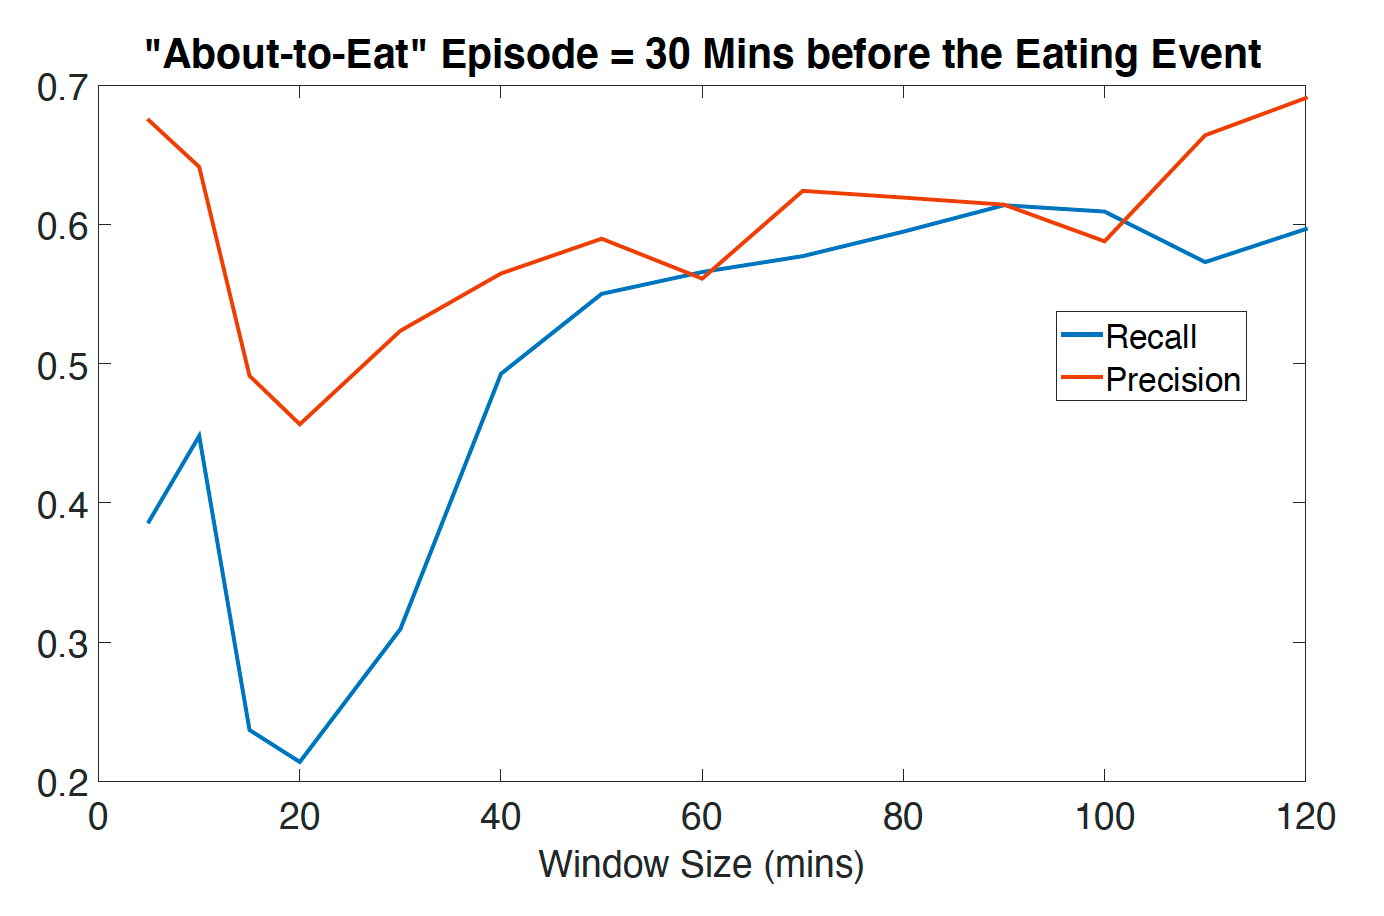
\includegraphics[width=0.5\textwidth]{./images/windowSizePerformance.png}
  \caption{This graph depicts the F measure with the different feature extraction window sizes of the "About-to-Eat" classifier.}
  \label{figure:windowSize}
\end{figure*}

The performance for the "Time until Next Eating Event" model gained a correlation coefficient of 0.49. The most fitting feature extraction window size was assessed, the best performance was reached with a window size of 100 minutes.
The authors further claim, that both models could be improved by incorporating person-dependent data from the target user to the models (e.g. person-specific eating pattern, lifestyle).




\textcite{SmartphoneBasedStressPrediction2015}[240, 242, ..] research, whether data collected by a user's smartphone can be used to predict stress. In their study, they used an android smartphone app called "TheStressCollector" (TSC) to collect smartphone usage and sensor data in the background. The following data was collected:
\begin{itemize}
  \item Activity: whether the device on the user is on foot, on a bike, in a vehicle, tilting, still or unknown.
  \item App Usage: apps for information, system, health, entertainment, social, or work
  \item Network Traffic: amount of network traffic (received and transmitted)
  \item Reboot Activity: power on and off events
  \item Calls: min, max and mean dB-values collected by the microphone
  \item Light: environment brightness
  \item Messages: timestamps of received messages
  \item Noise exposure: min, max and mean dB-values
  \item Screen Activity: duration of a user session (between screen power on and off)
\end{itemize}

15 participants installed the app on their smartphone and took part in the conducted study for two weeks. Seven times a day they would fill out questionaires (at set times), which included the perceived stress score (PSS) and queried them on their current stress status. The stress levels were predicted by WEKA'S machine learning algorithms. The mean absolute error (MAE) and Person correlation were used for the evaluation.The results of this study presented compelling correlations between PSS and the data collected by the smartphone app. The weekly PSS average, as opposed to the daily one, included the highest correlation coefficient. Thus, it is expected, that it easier to spot longer periods of high stress than shorter ones. 

customised brief version of the Perceived Stress Scale (PSS)

This paper also a team publication featured in the research project from which SmartEater was developed.








